\section{Aufbau}

Der Versuch wird mit einem D8-Diffraktometer durchführt, welches in Abbildung \ref{fig:aufbau} zu sehen ist. 

\begin{figure}
    \centering
    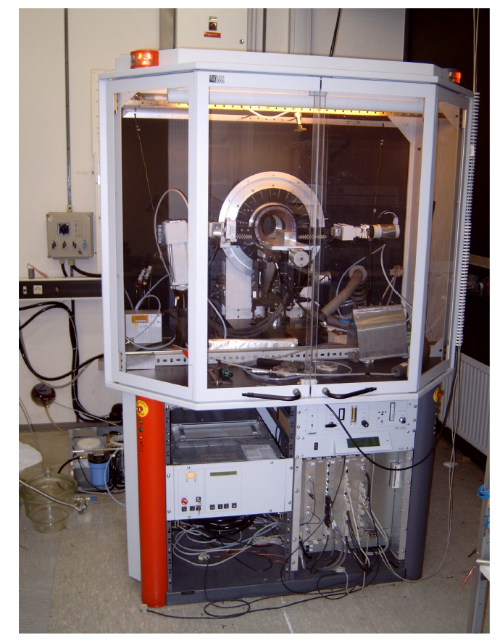
\includegraphics[scale=0.3]{content/D8.png}
    \caption{Das verwendete D8-Diffraktometer.\cite{Anleitung}}
    \label{fig:aufbau}
\end{figure} 

Dieses besteht aus einer Röntgenröhre mit Kupferanode, welche mit einer Spannung von $\SI{40}{\kilo\volt}$ und 
$\SI{40}{\milli\ampere}$ betrieben wird. Die austretende Strahlung trifft auf einen Göbelspiegel, der die Strahlung
bündelt und monochromatisiert. Der dann resultierende Strahl besitzt eine Wellenlänge von $\lambda = \SI{1.54}{\angstrom}$.
Die verwendete Röntgenröhre ist in Abbildung \ref{fig:rontgen} zu sehen. 

\begin{figure}
    \centering
    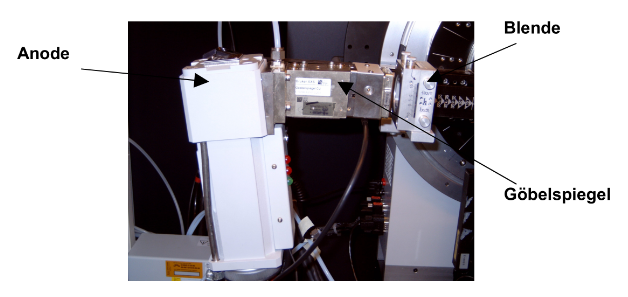
\includegraphics[scale=0.4]{content/rontgen.png}
    \caption{Röntgenröhre des D8-Diffraktometers.\cite{Anleitungalt}}
    \label{fig:rontgen}
\end{figure} 

\section{Durchführung}

Vor der eigentlichen Messung muss der Aufbau zunächst justiert werden. 

\subsection{Justage}

Für die Justage des Aufbaus sind sechs Schritte notwendig. 

\begin{description}
    \item[Detektorscan:]\hfill \\
    Zunächst wird die Probe aus dem Strahlgang entfernt. Es werden der Detektor und die Röntgenröhre auf Position $\SI{0}{\degree}$
    gefahren. Um nun die tatsächliche Nulllage des Detektors zu finden, wird nun seine Lage variiert, bis die Intensität des 
    Primärstrahls das Maximum durchläuft. Diese Position ist die neue Nullposition. 
    \item[Erster Z-Scan:]\hfill \\
    In diesem Schritt wird die Probenjustage angepasst. Um dabei die z-Position der Probe zu variieren, wird diese zunächst wieder
    in den Strahlgang geschoben. Dann wird die Intensität $I$ gemessen. Die Position der Probe wird variiert, bis $I$ auf den 
    Wert $I = \frac{1}{2}I_\text{max}$ gesunken ist. Der $z$-Wert wird notiert und die Motoren in die entsprechende Position 
    gebracht.
    \item[Erster Rockingscan:]\hfill \\
    Nun werden der Detektor und die Röntgenröhre um die Probe bewegt. Dabei wird ein konstanter Winkel zwischen der Probe und 
    dem Detektor mit $2\theta = \SI{0}{\degree}$ beibehalten. Die Drehung erfolgt dabei in einem Winkelbereich von $\SI{-1}{\degree}$
    bis $\SI{1}{\degree}$. Aus dem resultierenden Intensitätsverlauf wird dann das Maximum abgelesen und für die weiteren Schritte 
    verwendet. 
    \item[Zweiter Z-Scan:]\hfill\\
    Nach dem Rockingscan befindet sich die Probe nun nicht mehr in der gewollten Position. Aus diesem Grund wird ein erneuter 
    Z-Scan durchgeführt.
    \item[Zweiter Rockingscan:]\hfill\\
    Um eine Erhöhung der Präzession zu erreichen, wird ein erneuter Rockingscan mit $2\theta = \SI{0.3}{\degree}$ durchgeführt. 
    Es wird ein Scanbereich von $\SI{-0.5}{\milli\metre}$ bis $\SI{0.5}{\milli\metre}$ gewählt. Danach wird erneut das Maximum abgelesen
    und die Motoren entsprechend ausgerichtet.
    \item[Dritter Rockingscan:]\hfill\\
    Abschließend wird ein letzter Rockingscan mit $2\theta = \SI{1}{\degree}$ durchführt. Der Scanbereich wird als $\SI{0.45}{\degree}$
    bis $\SI{0.55}{\degree}$ gewählt, da das erwartete Maximum bei $\SI{0.5}{\degree}$ liegt. Das Maximum wird erneut abgelesen und 
    die Motoren entsprechend ausgerichtet.  
    
\end{description}

\subsection{Messung}

Nun wird ein Reflektivitätsscan durchgeführt. Bei diesem sind der Einfallswinkel $\alpha_i$ und der Winkel zwischen Probe 
und Detektor $\alpha_\text{f}$ gleich. Es wird ein Scanbereich von $\SI{0}{\degree}$ bis $\SI{5}{\degree}$ und eine Schrittweite 
von $\SI{0.05}{\degree}$ gewählt. Die Messzeit beträgt dabei pro Datenpunkt $\SI{5}{\second}$. \\
Außerdem wird ein diffuser Scan durchgeführt, bei dem der Anteil der gestreuten Intensität an der Reflektivität bestimmt wird. Dabei
gilt hier $\symup{\Delta}a = \vert \alpha_i - \alpha_\text{f}\vert = \SI{0.1}{\degree}$.